%
\documentclass[12pt,letterpaper]{article}
\usepackage{bbm}
\usepackage{url}
\usepackage{fancyhdr}
%\usepackage{fancybox}
%\usepackage{amstext}
\usepackage{amsmath}
%\usepackage{rotating}
\usepackage{multicol}
\usepackage{pictexwd}
\usepackage{enumitem}
%\usepackage{booktabs}
\usepackage{graphicx}
\usepackage{booktabs,multirow}
\usepackage{siunitx}

\setlength{\parindent}{0in}
\setlength{\textwidth}{7in}
\setlength{\evensidemargin}{-0.25in}
\setlength{\oddsidemargin}{-0.25in}
\setlength{\parskip}{.5\baselineskip}
\setlength{\topmargin}{-0.5in}
\setlength{\textheight}{9in}


%               Problem and Part
\newcounter{problemnumber}
\newcounter{partnumber}
\newcommand{\Problem}{\stepcounter{problemnumber}\setcounter{partnumber}{0}\item[\makebox{\hfil\textbf{\ \theproblemnumber.}\hfil}]}
\newcommand{\Part}{\stepcounter{partnumber}\item[(\arabic{partnumber})]}
\newcommand{\SubPart}{\stepcounter{problemnumber}\setcounter{partnumber}{0}}
\newcommand{\InPart}[1]{\stepcounter{partnumber}(\alph{partnumber})\ \ \parbox[t]{2.25in}{#1}}
\newcommand{\InSmallPart}[1]{\stepcounter{partnumber}(\alph{partnumber})\ \ \parbox[t]{1.05in}{#1}}

\pagestyle{empty}
\rhead{\large\texts{Angeline Baniqued \& Michael Wee}}
\lhead{\LARGE\textbf{CS 181: Assignment 2}}
\cfoot{}
\renewcommand{\headrulewidth}{0pt}

\begin{document}

\thispagestyle{fancy}\small

\setcounter{problemnumber}{0}
\begin{enumerate}

  \Problem \textbf{\textsc{\large{Perceptrons}}} \medskip
  
  \begin{enumerate}
    \Part bright-or-dark (At least $75$\%\ of the pixels are on, or at least $75$\%\ of the pixels are off.)\medskip

A perceptron cannot recognize this feature. A perceptron can easily be trained to recognize one of the two conditions, for example by having all of the weights be 1 and having a threshold activation function of either 7.5 or 2.5. However, once it is set to recognize one, it cannot recognize the other because the threshold would have been set at a hard limit already. \bigskip

        \Part top-bright (A larger fraction of pixels is on in the top row than in the bottom two rows) \medskip

A perceptron can recognize this feature. We can see this by having the three weights on the top row be $\frac{1}{3}$ and all the other six weights be $-\frac{1}{6}$.  We would set the threshold to 0 and check if the sum is greater than 0 to indicate a positive example and otherwise a negative example.\bigskip

        \Part connected (The set of pixels that are on is connected. (In technical terms, this means that if we define a graph in which the vertices are the pixels that are on, and there is an edge between two pixels if they are adjacent vertically or horizontally, then there is a path between every pair of vertices in the graph.)\medskip

A perceptron cannot detect this feature. There are too many variations and combinations in terms of number of pixels that are on as well as the location of where these pixels are. For example, 1 or 2 pixels on could be a path, as can 8 or 9. We cannot do anything with the total number of pixels on. We also cannot learn weights for specific squares or specific areas of the grid because paths can appear in any location. So any way we train the weights we can come up with a counter example path that the weight set incorrectly classifies by countering the training strategy. This means either by changing the number of pixels that are on, or constructing a path on a different portion of the grid than where the weights were originally tuned to correctly classify paths. 
 
 
       
        
  \end{enumerate}
  \bigskip 

  \Problem \textbf{\textsc{\large{Learning Algorithms} }} \medskip 
  \begin{enumerate} 
    \Part The domain of handwritten digit recognition is 14x14 pixels with intensities ranging from 0 to 255. The features for this domain are the pixel intensities themselves.

\begin{itemize}
\renewcommand{\labelitemi}{$\bullet$}
\item Decision trees \medskip

        Decision trees that are modified to split on ranges of continuous values would be able to classify handwritten digits though they will neither be as effective nor as natural for this domain as other techniques such as using neural networks. The decision tree would need an effective algorithm to take into account lookahead because digit recognition revolves around combinations of pixel intensities. An algorithm analogous to ID3 would not work well because of the reliance of attributes on one another and the fact that nearby pixels affect recognition of what digit is formed. Because of the relatively large number of pixels, an effective decision tree would have to be deep because they would have to predict on combinations of features, not single attributes.  Decision trees would also have to be pruned since their tendency to overfit combined with many features (as well as the possibility to split more than once on any given continuous attribute).  \\
        While decision trees conceivably could be constructed to do well on digit recognition, it does not lend itself naturally to this domain. An analogous algorithm to ID3 would fail miserably. So while there are decision trees that can classify the digits and though we're sure there may be algorithms that adequately do lookahead and attribute combinations, but there are more natural choices for this domain that requires combinations of features to be effective. \medskip


\item Boosted decision stumps \medskip

        Boosted decision stumps wouldn'�t do well on this domain. Because boosted decision stumps split on only one attribute, they do not combine features and individually will not be able to capture patterns in the data well enough to classify digits. Individual stumps can do no better than chance since on their own they cannot predict what digit a particular pixel intensity is a part of. \medskip
\item Perceptrons \medskip

        Perceptrons would be especially bad for recognizing digits. Since there are 10 possible digits to correctly classify, it presents too much variability for a single perceptron to classify. Perceptrons have more limitations beyond just being able to output binary values, which is a problem in a 10-class domain. \medskip

\item Multi-layer feed-forward neural networks \medskip

        Multi-layer feed-forward neural networks are very suited for the domain of recognizing hand written digits. Because the digits are represented as a matrix of pixels, a neural network can propagate pixel intensities and calculate a decision boundary based on combinations of all of these features. 
        Moreover, the flexibility in designing feed-forward networks lends itself even further to classifying digits, allowing for custom hidden layers to compute and pass forward useful features like averaging/subsampling and feature maps downstream.\bigskip




  \end{enumerate}
  \bigskip 
  
  \Problem \textbf{\textsc{\large{Neural Networks}}} \medskip
        \begin{enumerate}
        \Part See FeedForward function.\medskip
        \Part See Backprop function.\medskip
        \Part See Train function.\medskip
        \Part See EncodeLabel, GetNetworkLabel, Convert and InitializeWeights  functions.\medskip 
        \Part Input data normalization is useful when we think about the shape of the sigmoid function which is the activation function we use. The sigmoid function is approximately linear when input is near 0 and converges to 1 for large input and 0 for small input. Since the activation/sigmoid function takes in the linear combination of weights and activity at each parent node, we want that linear combination to be in the vicinity of 0 which can be achieved by normalizing the input values from [0,255] to between [0,1]. \medskip

        Furthermore, if we have a wide range of input values, the bigger values will tend to
have a higher contribution to the output error, and so, the error reduction algorithm will
be focused on the higher values, neglecting the information from the small
valued variables. 
        \medskip
         
        \Part Simple Network \medskip
               \begin{enumerate}[label={\alph*)},ref={\alph*)}]
                \item \textbf{Chosen learning rate = 1.0} \medskip
                \item Chart of Training Set and Validation Set Error vs. Number of Epochs\\
                        \includegraphics[width=5in]{simple_1p0.png}
                         \begin{enumerate}[label={\roman*)},ref={\roman*)}]
                                \item Like other statistical models, neural networks are also subject to overfitting. By looking at the plot of the number of epochs of training on the x-axis, and the classification error on the y-axis, we see the standard overfitting phenomenon. \medskip
                                \item From the plot, the classification error on the validation set increases at around epoch 23, so we could train for 23 epochs and then stop there. \medskip 
                                \item It's useful to divide the dataset into three (train, validation and test) because each set serves an important purpose. We need the training set to actually train the neural network, but then during training, the classification error on the training set will continue to decrease as the number of epochs increases due to overfitting. Thus, we need the validation set because there will be some point after which we will be overfitting and we can detect overfitting by looking at when the validation set increases. It's important to use the validation set instead of the test set because (1) we shouldn't be peeking at the test data because the test set should be set aside for when we want to 'test' a non-overfitting neural network  and (2) without a validation set, we wouldn't be able to find a non-overfitting neural network to test. \medskip
                        \end{enumerate} 
                \item This training rate\ of 1.0 produced the highest performance on the training, validation and test sets: \\  Training set performance = 0.89\\
                      Validation set performance = 0.87\\
                      Test set performance = 0.91
                      \bigskip                     
               \end{enumerate} \medskip
               \end{enumerate}

                For reference and comparison, here are the results of the other learning rates that we didn't end up choosing\ (0.1, 0.01, 0.001). 
               \begin{enumerate}[label={\alph*) },ref={\alph*)}]
               \item \textbf{Learning rate = 0.1} \medskip
                \item Chart of Training Set and Validation Set Error vs. Number of Epochs \\
                        \includegraphics[width=5in]{simple_0p1.png}
                        \begin{enumerate}[label={\roman*)},ref={\alph*)}]
                                \item same answer as in the 1.0 learning  rate case \medskip
                                \item From the plot, the classification error on the validation set increases at around epoch 14, so we could train for 14 epochs and then stop there. \medskip 
                                \item same answer as in the 1.0 learning rate case
                        \end{enumerate} 
                        \bigskip
                \item Training set performance = 0.88\\
                      Validation set performance = 0.87\\
                      Test set performance = 0.91
                      \bigskip
                \end{enumerate} \medskip
                
                \begin{enumerate}[label={\alph*) },ref={\alph*)}]
               \item \textbf{Learning rate = 0.01} \medskip
                \item Chart of Training Set and Validation Set Error vs. Number of Epochs\\
                        \includegraphics[width=5in]{simple_0p01.png}
                        \begin{enumerate}[label={\roman*) },ref={\alph*)}]
                                \item same answer as in the 1.0 learning  rate case \medskip
                                \item From the plot, the classification error on the validation set increases at around epoch 19, so we could train for 19 epochs and then stop there. \medskip
                                \item same answer as in the 1.0 learning rate case \medskip

                        \end{enumerate} 
                        \bigskip
                \item Training set performance = 0.87 \\
                      Validation set performance = 0.86 \\
                      Test set performance = 0.91
                      \bigskip
                \end{enumerate}  \medskip
                
                \begin{enumerate}[label={\alph*) },ref={\alph*)}]
               \item \textbf{Learning rate = 0.001} \medskip
                \item Chart of Training Set and Validation Set Error vs. Number of Epochs\\
        \includegraphics[width=5in]{simple_0p001.png}     \\
                    \begin{enumerate}[label={\roman*)},ref={\alph*)}]
                                 \item same answer as in the 1.0 learning  rate case \medskip
                                \item From the plot, since the learning rate is so small, we might require a greater number of epochs (greater than 100) to see the overfitting phenomenon more clearly. \medskip
                                \item same answer as in the 1.0 learning rate case \medskip
                        \end{enumerate} 
                        \bigskip
                \item Training set performance = 0.86 \\
                      Validation set performance = 0.85\\
                      Test set performance = 0.90
                      \bigskip
                \end{enumerate} \bigskip
          \Part Hidden Network \medskip
                \begin{enumerate}[label={\alph*) },ref={\alph*)}]
                \item We used 1.0, 0.1, 0.01, and 0.001 as the learning rates for both 15 and 30 hidden units. We chose these rates in order to find the order of magnitude of the most effective learning rate. \medskip \\
                For both 15 and 30 hidden units, we found that the optimal learning rate was on the order of 0.1. Test/train/validation performances are mentioned in the succeeding subproblems. The learning rate of 1.0 caused oscillations in gradient descent and didn't really converge whereas the small learning rates of 0.01 and 0.001 cause gradient descent to converge really slowly.  
\medskip
                \item We monitor the validation set performance of the neural network. Our stopping condition is when the validation set performance decreases twice in a row. Empirically we found that a one-time decrease in validation was not enough to guarantee a good stopping point and a three-in-a-row decrease in validation performance rarely occurred in general. (We implemented this rule in the Train function in $neural\_net.py$).\                        \medskip
                \item Chart of Training Set and Validation Set Error vs. Number of Epochs (15 hidden units) \medskip 
                \includegraphics[width=5in]{hidden15_0p1_zoomed.png} 
                
                Chart of Training Set and Validation Set Error vs. Number of Epochs (30 hidden units) \medskip 
                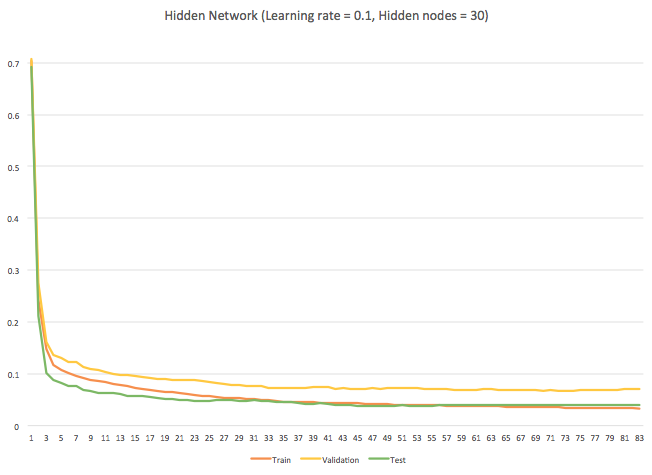
\includegraphics[width=5in]{michael-part/hidden30-1.png}
                \item For 15 hidden units with learning rate 1.0, we stopped after 10 epochs (2 consecutive decreases after). With the \textbf{optimal} learning rate 0.1, we stopped after 54 epochs. With learning rate 0.01, we stopped near 100 epochs (might need more than 100 epochs). With the optimal learning rate 0.001, we stopped near 100 epochs\ (might need more than 100 epochs).\medskip

For 30 hidden units with learning rate 1.0, we stopped after 6 epochs (2 consecutive decreases after). With the \textbf{optimal} learning rate 0.1, we stopped after 79 epochs. With learning rate 0.01, we stopped after 83 epochs. With learning rate 0.001, we stopped after 83 epochs.          \medskip
                \item For 15 units, using optimal learning rate 0.1 and stopping after 54 epochs, we get train performance of 0.94, validation performance of 0.91, and  test performance of 0.935.
\medskip \\
For 30 units, using optimal learning rate 0.1 and stopping after 79 epochs, we get train performance of 0.97, validation performance of 0.93, and test performance of 0.961.\medskip \\
By comparing the two, we would choose the network structure of 30 hidden units given that it outperforms the 15 units network structure on all the training, validation and test sets. 
                        \medskip
                \item The test set performance of our chosen network with 30 hidden units and an optimal rate of 0.1  is 0.961 as mentioned above. This does significantly better than the test set performance of the committee of perceptrons with learning rate 1.0 in 3.6 which hovered around 0.91.
                \bigskip
                \bigskip
                \end{enumerate}
          \Part Hidden Network \medskip
          \begin{enumerate}[label={\alph*)},ref={\alph*)}]
                \item We experimented with adding a fully connected second hidden layer with various numbers of hidden units. We ran experiments letting the two hidden layers have the same number of hidden units, ranging from a small number of hidden units to a larger number of hidden units. We also experimented with varying the number of hidden units in each layer, for example having 10 in the first and 15 in the second. \\

Having achieved success with one layer, we thought we could improve on this success by adding another hidden layer. We reasoned that the automatic feature engineering intuition associated with neural networks would result in the first hidden layer passing the second hidden layer an even better set of features which the second hidden layer can then do learning on.  \\

One other set of experiments we ran, based on the intuition we get from the previous section, is increasing the number of hidden nodes in the single hidden layer. It makes sense that more hidden nodes (as long as they are still on the order of the number of input and output nodes) would be able to do more with the data and should do better.  \\

We ran all of our experiments with a learning rate for 0.1 that we found to be optimal for hidden layer training above.

\medskip \\
                \item The neural networks we trained with two hidden layers universally start with very poor performance on training, validation, and test sets. For the experiments we ran with more 25 total hidden nodes or nodes, all had training error, validation set error, and test error at 0.12 or worse for the first 30 or so epochs before starting to improve. In fact, the errors only change once in a while in the first 30 epochs indicating that weights were not necessarily being changed in a way that would change the way classification was done. However, after the first 30 or so epochs, performance quickly increases to the level of one hidden unit and continues to increase. \\
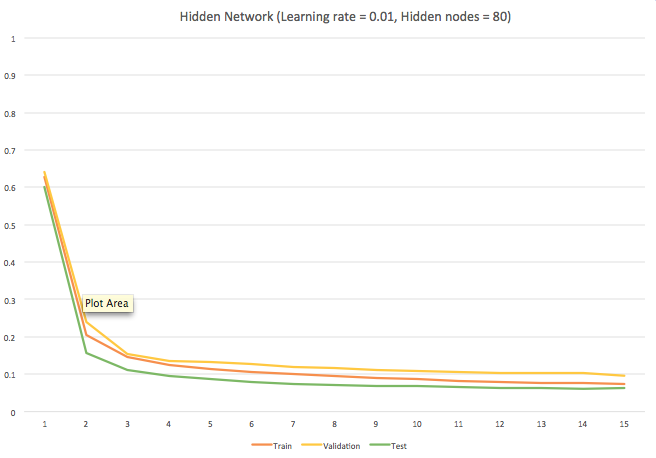
\includegraphics[width=5in]{michael-part/1_layer_80.png} \medskip \\
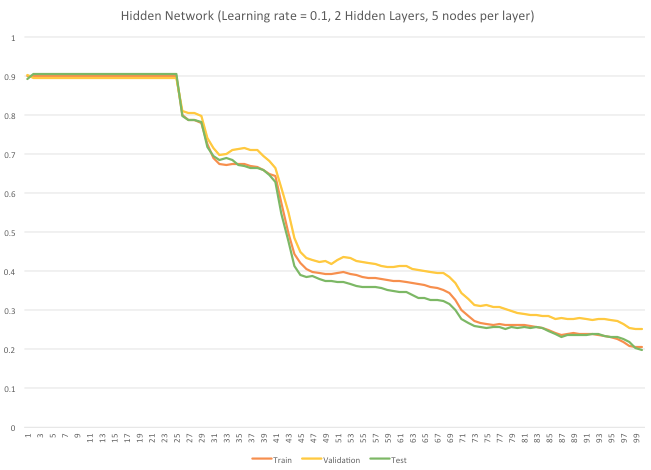
\includegraphics[width=5in]{michael-part/2_layer_5.png} \medskip \\
        Because, unlike LeCun et al, we did not do feature engineering with the extra hidden layers we had, the actual benefit of having an extra hidden layer may be small because each hidden layer was assigned just a general task to update weights as best as it can. In fact, because each hidden layer was only given instructions to learn the general structure, in the first 30 epochs it may have taken a lot of time to figure out exactly what kinds of the results the first layer should be passing to the second layer and how the second layer should interpret them, leading to inferior results for a while. Also, because the number of weights increases quadratically with the number of hidden units adding two layers increases the number of weights to train as well. Having more than one hidden layer also makes the neural network more susceptible to local minima and our particular algorithm does not deal with escaping from and searching around local minima. Our experiments with two hidden layers with 10 total units and learning rate 0.1 peaked out at 0.8 test error after 100 epochs, but the network was still steadily increasing performance. This might be because there are fewer hidden nodes to learn hypotheses with, but also more complex interplay between the two layers, requiring more epochs to learn a good network. The case where we varied the number nodes in each layer (say 10 and 15 versus 15 and 15) and similar performance to having the same number of nodes in each hidden layer. \\

        Having two hidden layers without special engineering may also not be necessarily better because the second hidden layer works with values that are summed and then passed through the sigmoid function which changes the distribution of values. In addition, classification now depends on the weighted output of the second layer, which in turn depends on the weighted outputs of the first layer. With all nodes feeding in to each other this could create a situation where there is a lot of interplay or interference in between layers. From this experiment we conclude that without careful feature engineering, additional hidden layers should be added with care and must be carefully tuned to have a good learning rate so that we prevent the long wait in the first 30 or so epochs with little results. \\ 
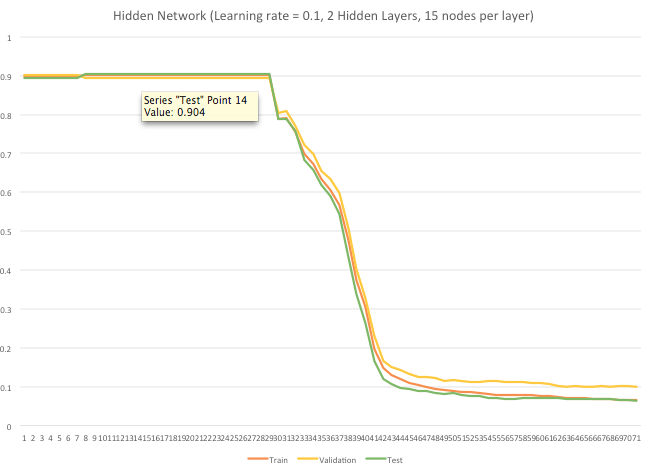
\includegraphics[width=5in]{michael-part/2_layer_15.png} \medskip \\
        Our experiments with a single hidden layer with a large number of nodes yielded promising results. We ran a network with 80 hidden units and 150 hidden units overnight and saw the following results. With both 80 and 150 hidden units, the test performance increases very rapidly within 4 epochs to have test performance of over 0.9. Test performance then monotonically increases for the 15 epochs or so we were able to train (having this many hidden nodes takes a long time to train because number of weights to train increases quadratically with number of units). Validation set performance also steadily increases. With learning rate 0.1, the network with 80 units does very slightly better on test performance while the network with 150 units does very slightly better on validation set performance. Both networks do similarly to the network with 30 hidden units for the first 15 or so epochs, sometimes one doing slightly better on the validation set, sometimes the other doing slightly better on the test set. We expect that slightly more hidden nodes will do better in the long run as it can learn more complex hypotheses while still being regulated for overfitting by the validation set stopping rule.
        

                        \medskip
                \bigskip
                \end{enumerate}
        \end{enumerate}
     \bigskip \\
  
  \Problem \textbf{\textsc{\large{Alternative Error Function}}} \medskip
        \begin{enumerate}
        \Part The difference between the error function $C$ and the loss function $L$ is that the former implements some kind of regularization that  penalizes  large $w_{km}$ and $w_{mj}$ weights. Since we're trying to minimize $C$, we would also want to minimize the magnitude  of $w_{km}$ and $w_{mj}$.\medskip
\\ The added penalty terms cause the weights to converge to smaller
magnitudes than they otherwise would. Large weights can hurt
generalization in a number of ways. Extremely large weights from input to
hidden units and extremely large weights from hidden to output units can
cause greater variance in outputs  beyond the range of the data if the activation
function does not have the same range as the input data. This error function $C$ prevents the network from using weights that it does not need, from overfitting the noise in the data and from stretching the variance of outputs too much. 
        \medskip
        \Part \medskip
        $$ C(w)  = \displaystyle\sum_{n=1}^{N}\sum_{j=1}^{J}(y_{nj}-a_{nj})^2 + \lambda \sum_{m=1}^{M}\left( \sum_{k=0}^{K} w_{km}^2 + \sum_{j=1}^{J} w_{mj}^2\right) $$

        For updating weights $w_{km}$ between input $k$ and hidden input $m$, for a particular example, we have: 

        $$\displaystyle \frac{\partial{ C(w)}}{\partial w_{km}} &= \displaystyle \frac{\partial{}}{\partial w_{km}} \left(\sum_{j=1}^{J}(y_{j}-a_{j})^2\right) + \lambda \displaystyle \frac{\partial{}}{\partial w_{km }}\left( \sum_{m'=1}^{M} \sum_{k'=0}^{K} w_{k'm'}^2 \right) + \lambda \displaystyle \frac{\partial{}}{\partial w_{km }}\left( \sum_{m'=1}^{M} \sum_{j'=1}^{J} w_{m'j'}^2 \right)$$\\
The first term on the right-hand side is exactly the same as that in the loss function. We've derived the partial derivative on the first term in the Lecture 6 notes on page 9. \medskip\\ The last term or partial derivative on the right-hand side of the equation is just $0$ since $w_{km}$ doesn't appear in the expression $w_{m'j'}^2$. Thus, we only have to simplify the middle term. In the middle term, the weight $w_{km}$ only influences the $m$th hidden unit, so only one element in the summation matters. Simplifying, we get the following gradient descent:  
  \begin{equation*}
  $ \displaystyle  &= -2g'(z_m)x_k  \sum_{j=1}^{J} \delta_{j}w_{mj} + \lambda 2 w_{km}$ \medskip \\
 $ \propto \left(a_k\delta_m + \lambda w_{km}\right)   
  \end{equation} \medskip \\ 
 
 Deriving a weight update rule, we get $w_{km}^{(r+1)} \leftarrow w_{km}^{(r)} +\alpha\left(a_k\delta_m + \lambda w_{km}^{(r)}\right).$ Combining terms and constants, we have, $w_{km}^{(r+1)} \leftarrow (1 +\lambda')w_{km}^{(r)} +\alpha\left(a_k\delta_m \right) $. The $\lambda'$ can be determined using cross validation. \bigskip

For updating weights $w_{mj}$ between hidden unit $m$ and output $j$ for a particular example, we take the partial derivatives with respect to $w_{mj}$, go through the same process and arrive at the following similar weight update rule: $w_{mj}^{(r+1)} \leftarrow (1 +\lambda')w_{mj}^{(r)} +\alpha\left(a_m\delta_j \right) $ .

        
        \end{equation}

          
        \end{enumerate}
    \bigskip \\

\end{enumerate}

        

  \end{enumerate}

  \bigskip
  
 
\end{enumerate}
\end{document}
